\documentclass[tikz,border=10pt]{standalone}

\usepackage{tikz}
\usetikzlibrary{positioning}
\usetikzlibrary{shapes,arrows,backgrounds,fit,shapes.geometric,calc}
\usetikzlibrary{pgfplots.groupplots}
\usepackage{pgfplots}
\usepackage{pgfplotstable}
\usepackage{listings}
\usepackage{lstautogobble}
\usepackage{color}
\usepackage{amsmath}

\lstset{
    language=[ANSI]C++,
    basicstyle=\small\ttfamily,
    identifierstyle=\color{black}\small\ttfamily,
    keywordstyle=\color{red}\small\ttfamily,
    commentstyle=\color{green!30!black}\bf\small\ttfamily,
    breaklines=true
}

\tikzset{
    %Define standard arrow tip
    >=stealth',
    % Define arrow style
    pil/.style={
           ->,
           thick,
           shorten <=2pt,
           shorten >=2pt,}
}

\newcommand{\nodewidth}{1cm}
\newcommand{\nodeheight}{1cm}
\newcommand{\memwidth}{12cm}
\newcommand{\memheight}{2cm}
%\newcommand{\vin}[1]{$\text{in}_{#1}$}
\newcommand{\vin}[1]{${#1}$}
\newcommand{\vout}[1]{${#1}$}

\begin{document}
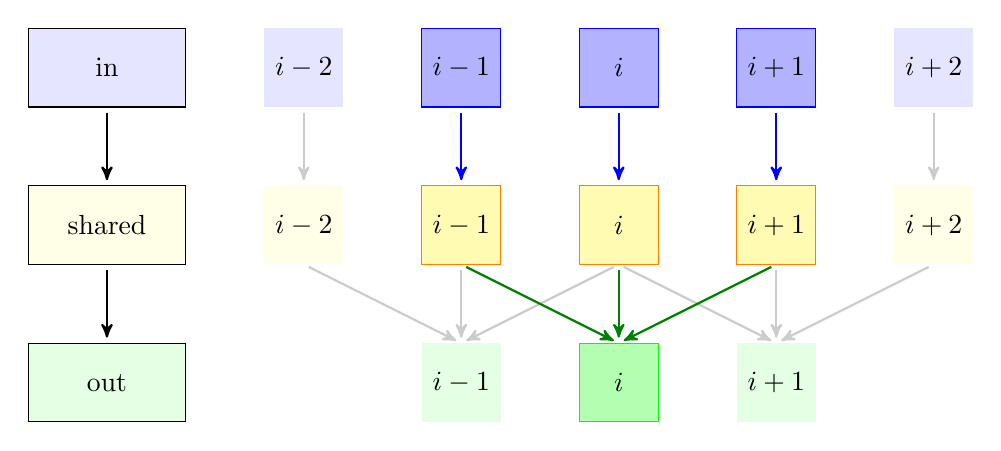
\begin{tikzpicture}[x=0cm, y=0cm, node distance=0 cm,outer sep = 0pt]
\tikzstyle{nin}=[ draw=blue,
                  rectangle,
                  minimum height=\nodeheight, minimum width=\nodewidth,
                  fill=blue!30,
                  anchor=north west]
\tikzstyle{ninm}=[
                  rectangle,
                  minimum height=\nodeheight, minimum width=\nodewidth,
                  fill=blue!10,
                  anchor=north west]
\tikzstyle{nbuff}=[ draw=red!50!yellow,
                  rectangle,
                  minimum height=\nodeheight, minimum width=\nodewidth,
                  fill=yellow!30,
                  anchor=north west]
\tikzstyle{nbuffm}=[
                  rectangle,
                  minimum height=\nodeheight, minimum width=\nodewidth,
                  fill=yellow!10,
                  anchor=north west]
\tikzstyle{nout}=[ draw=green,
                  rectangle,
                  minimum height=\nodeheight, minimum width=\nodewidth,
                  fill=green!30,
                  anchor=north west]
\tikzstyle{noutm}=[
                  rectangle,
                  minimum height=\nodeheight, minimum width=\nodewidth,
                  fill=green!10,
                  anchor=north west]

\tikzstyle{lab}=[ rectangle,
                  minimum height=\nodeheight, minimum width=2 cm,
                  anchor=north west]

\node[ninm] (inm2) at(0,0) {\vin{i-2}};
\node[nin]  (inm1) [right = 1cm of inm2] {\vin{i-1}};
\node[nin]  (in)   [right = 1cm of inm1] {\vin{i}};
\node[nin]  (inp1) [right = 1cm of in]   {\vin{i+1}};
\node[ninm] (inp2) [right = 1cm of inp1] {\vin{i+2}};

\node[nbuffm]  (buffm2) [below = 1cm of inm2] {\vout{i-2}};
\node[nbuff]  (buffm1) [below = 1cm of inm1] {\vout{i-1}};
\node[nbuff]  (buff)   [below = 1cm of in]   {\vout{i}};
\node[nbuff]  (buffp1) [below = 1cm of inp1] {\vout{i+1}};
\node[nbuffm]  (buffp2) [below = 1cm of inp2] {\vout{i+2}};

\path[pil,->,white!80!black] (inm2.south)  edge (buffm2.north);
\path[pil,->,blue] (inm1.south)  edge (buffm1.north);
\path[pil,->,blue] (in.south)    edge (buff.north);
\path[pil,->,blue] (inp1.south)  edge (buffp1.north);
\path[pil,->,white!80!black] (inp2.south)  edge (buffp2.north);

\node[noutm]  (outm1) [below = 1cm of buffm1] {\vout{i-1}};
\node[nout]   (out)   [below = 1cm of buff]   {\vout{i}};
\node[noutm]  (outp1) [below = 1cm of buffp1] {\vout{i+1}};

\path[pil,->,white!80!black] (buffm2.south)  edge (outm1.north);
\path[pil,->,white!80!black] (buffm1.south)  edge (outm1.north);
\path[pil,->,white!80!black] (buff.south)    edge (outm1.north);

\path[pil,->,white!80!black] (buffp2.south)  edge (outp1.north);
\path[pil,->,white!80!black] (buffp1.south)  edge (outp1.north);
\path[pil,->,white!80!black] (buff.south)    edge (outp1.north);

\path[pil,->,green!50!black] (buff.south)  edge (out.north);
\path[pil,->,green!50!black] (buffm1.south)  edge (out.north);
\path[pil,->,green!50!black] (buffp1.south)  edge (out.north);

\node[lab] (inlab) [draw, fill=blue!10, left = 1cm of inm2] {in};
\node[lab] (bufflab) [draw, fill=yellow!10, below = 1cm of inlab] {shared};
\node[lab] (outlab)  [draw, fill=green!10,  below = 1cm of bufflab] {out};
\path[pil,->,black] (inlab.south)  edge (bufflab.north);
\path[pil,->,black] (bufflab.south)  edge (outlab.north);


\end{tikzpicture}

\end{document}

